\section{Data Analysis of De-Noising data with AI assistance}

The two data samples, background merged and de-noised, were also processed with new 
reconstruction software, which includes AI assisted track candidate identification~\cite{Gavalian:2020oxg},\cite{Gavalian:2020xmc}. 
The reconstruction software is designed to be able to process data in two parallel branches, where in one 
branch it reconstructs tracks with conventional algorithm where track candidates are identified by fitting all 
combinations of clusters forming a candidate and choosing candidates that pass the ``goodness'' of the fit criteria, 
 and on the second branch AI classifies track from the list of candidates crated from all combinations of clusters 
 forming a track. 
 %This procedure is described in detail in~\cite{Gavalian:2022hfa}. 
 The details on track candidate identification, software implementation and resulting outcome for increased 
 track reconstruction efficiency can be found in~\cite{Gavalian:2022hfa}.
 Two samples were processed and comparison was made between conventional tacking algorithm from raw 
 background merged files, and output of de-noised data sample with and without AI assisted tracking. 

\subsection{Luminosity dependence}

The track reconstruction efficiency was calculated for three samples using Eq.~\ref{eq::eff}.
The results are presented on Figure~\ref{lscan::conv_dn_ai}. It can be seen from the figure that using 
AI assisted tracking on de-noised data sample further improves reconstruction efficiency. The raw background 
merged data sample exhibits tracking efficiency decline of $0.23\%$ per nA, while the combination of de-noising 
and AI assisted tracking reduces this slope to $0.12\%$ per nA (almost factor of 2), resulting in efficiency of $0.86\%$ at
 beam current $150~nA$ compared to $0.88\%$ at $45~nA$ beam current. 

\begin{figure}[!h]
\begin{center}
 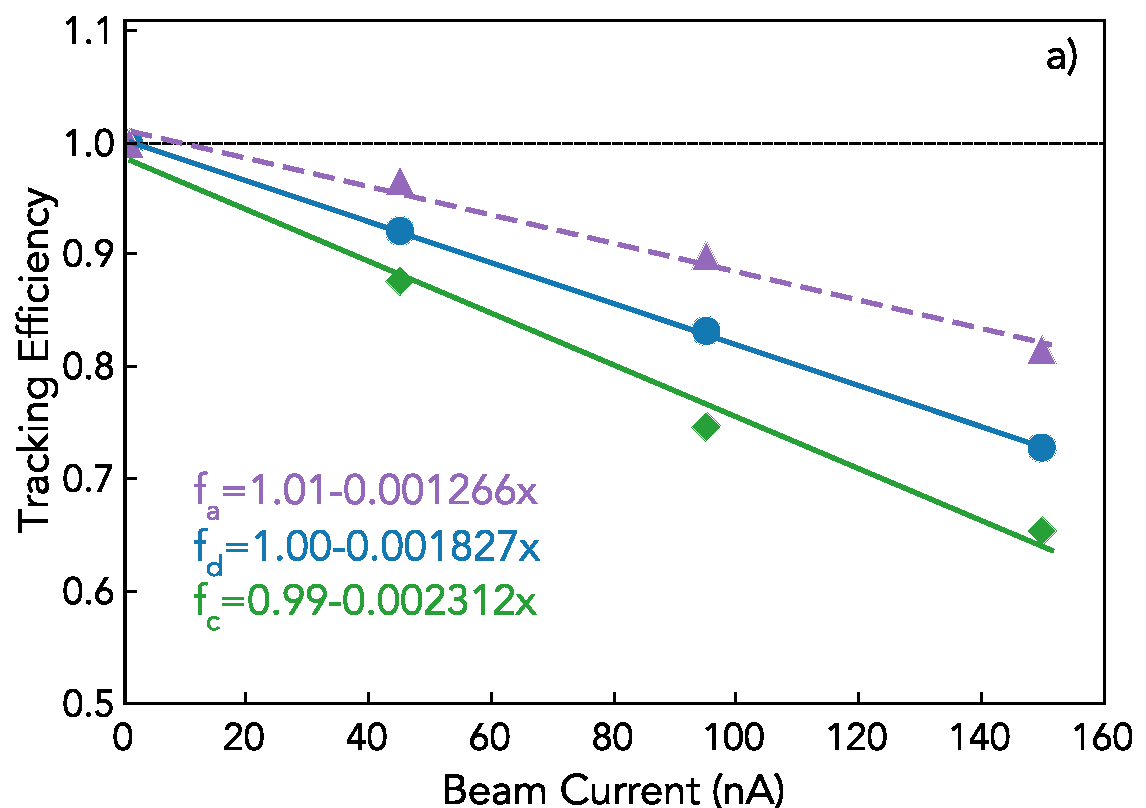
\includegraphics[width=3.1in]{images/figure_lscan_pos_ai.pdf}
 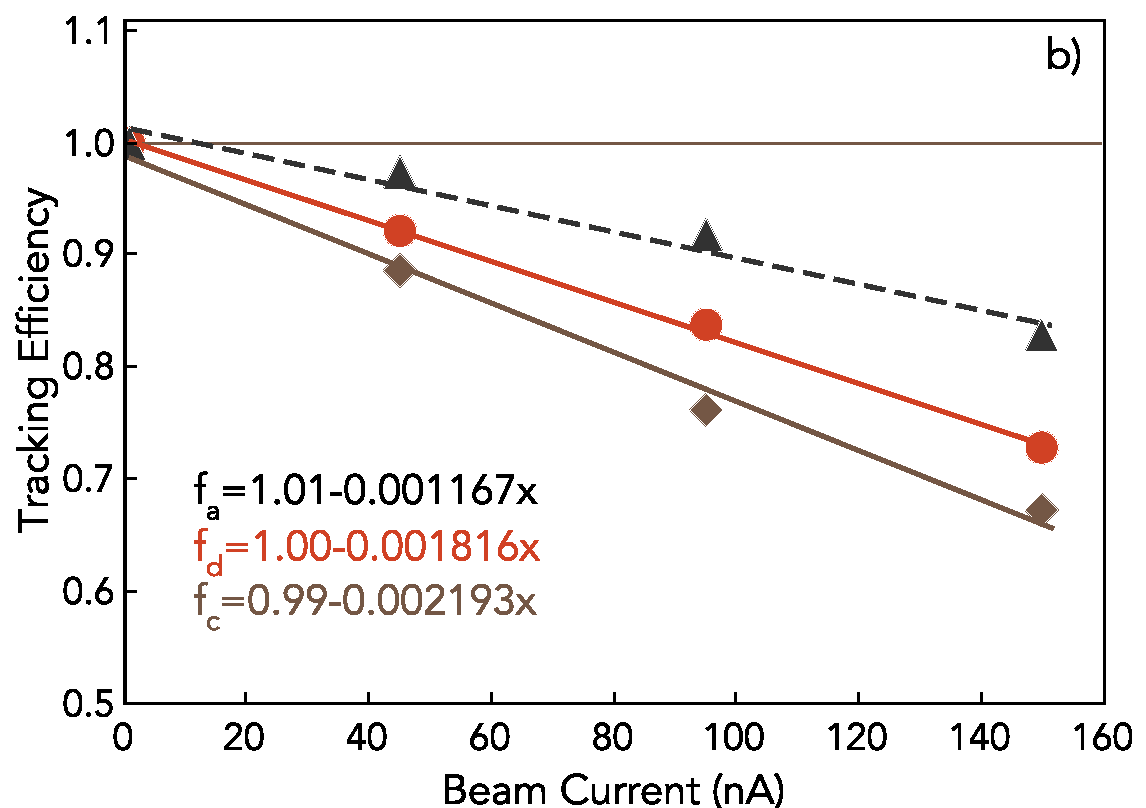
\includegraphics[width=3in]{images/figure_lscan_neg_ai.pdf}
\caption {Tracking efficiency as a function of luminosity (beam current) for positive (a) and negative particle (b).  The efficiency is shown for
conventional algorithm running on background merged files (diamonds), and on files with merged background then de-noised with AI (circles).}
 \label{lscan::conv_dn_ai}
 \end{center}
\end{figure}

This is significant improvement in tracking efficiency when using both AI assisted tracking with de-noising for beam current 3 times higher than current data collecting conditions. 

\subsection{Physics Impact}

Further the physics impact was studied for de-noised data sample processed with AI assisted tracking. Same data 
sample was used in this studies with selected $H(e,e^-\pi^+\pi^-p)X$ event from Pythia simulations, and analyzed for
missing mass of $H(e,e^-\pi^+\pi^-)X$, where number of protons were extracted from under the missing mass. 


\begin{figure}[!h]
\begin{center}
 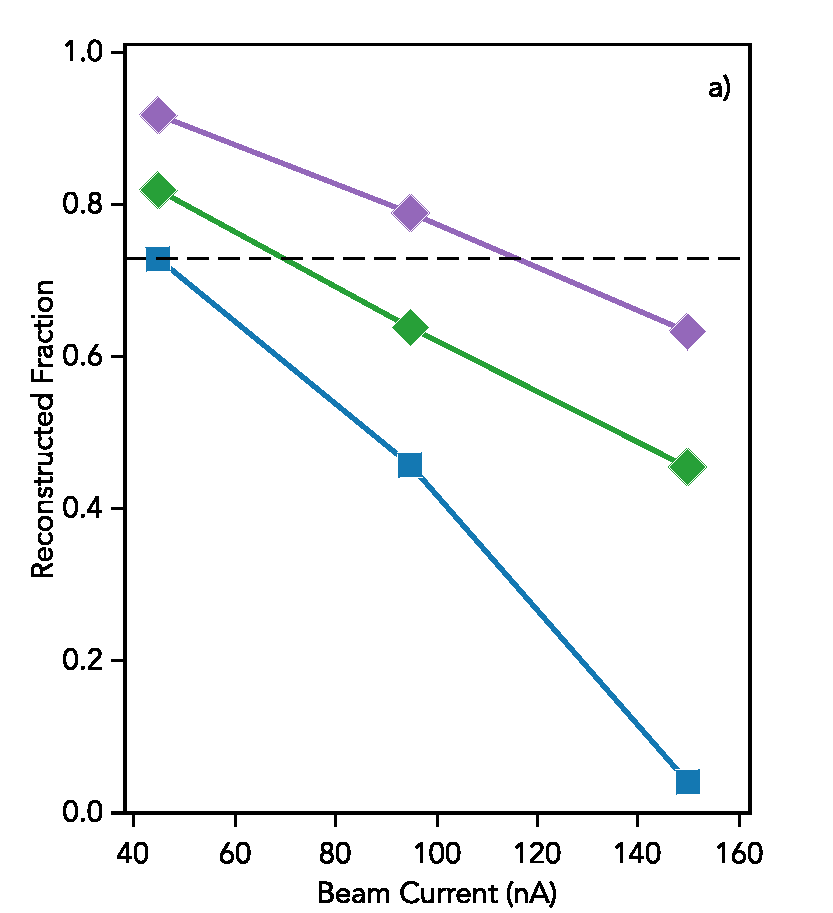
\includegraphics[height=3.1in]{images/graph_mxepipi_dn_ai.pdf}
 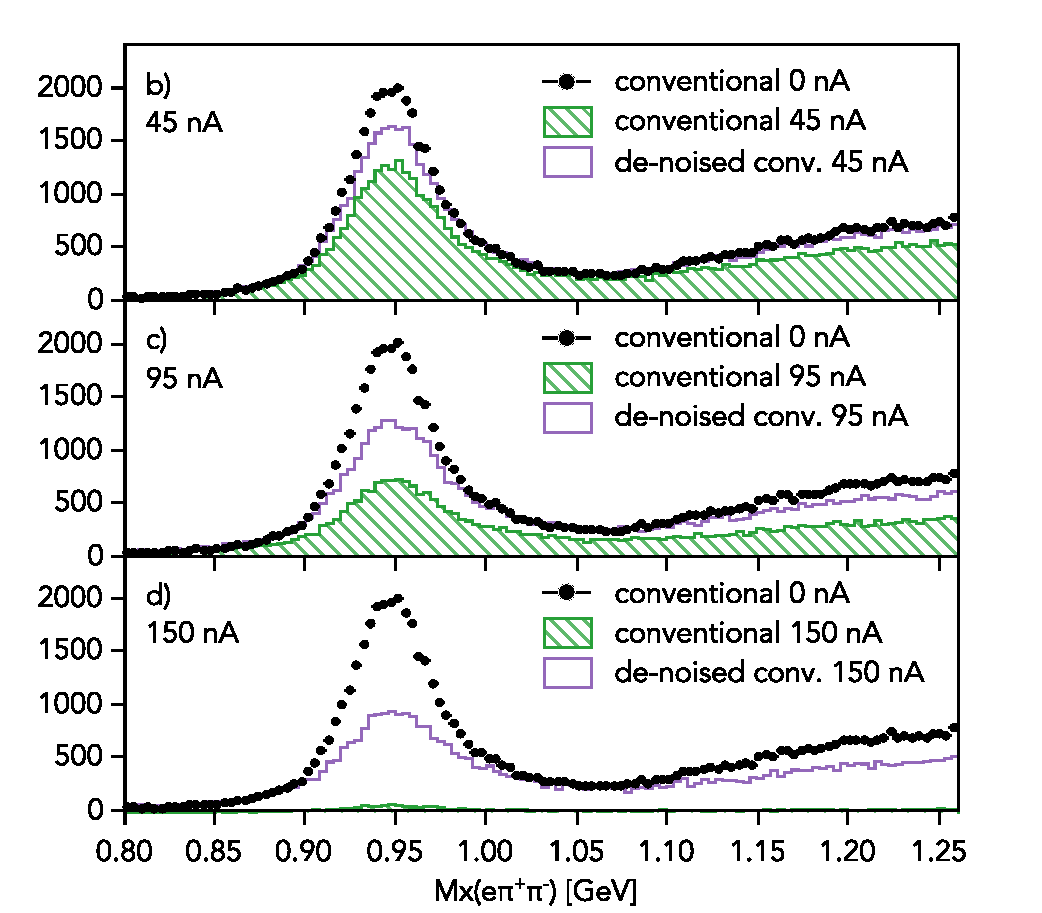
\includegraphics[height=3.1in]{images/plots_mxepipi_dn_ai.pdf}
\caption { a) Number of reconstructed protons from missing mass of $H(e \rightarrow e^\prime \pi^+\pi^-)X$ 
for background merged data set reconstructed with conventional tracking (squares) compared to de-noised data sample 
reconstructed with conventional algorithm (diamonds) and de-noised data sample reconstructed with AI assisted tracking 
algorithm (triangles)  for $45~nA$, $95~nA$ and $150~nA$. b), c) and d) reconstructed missing mass distributions for 
background merged data set reconstructed with conventional tracking (filled histogram) and de-noised data sample 
reconstructed with AI assisted algorithm (solid line histogram). Missing mass distribution for data sample before 
background merging ($0~nA$) is shown (circles) for reference. }

 \label{physics::conv_dn_ai}
 \end{center}
\end{figure}

The distributions of missing mass spectra are shown In Figure~\ref{physics::conv_dn_ai} for different beam current backgrounds.
In b), c) and d) the missing mass distributions are shown for background merged data samples processed with conventional algorithm 
(filled histogram) and reconstructed missing mass after data de-noising and reconstructing with AI assisted tracking (line histogram).
The graphs (circle symbol) on all three plots show missing mass distribution reconstructed from generated data sample 
before any background is added for reference. In Figure~\ref{physics::conv_dn_ai} a) the summary of the studied data samples 
are presented. The background merged data samples analyzed with conventional tracking algorithm (squares) show sharp decline in
number of reconstructed protons under the missing mass peak. Pre-processing data with de-noising auto-encoders and processing
with conventional algorithm (diamonds) improves the physics outcome due to improved single track efficiency. The biggest improvement
comes from using AI assisted track classification software after de-noising the drift chamber data (triangles). 

%The top row of plots shows missing mass distributions for different backgrounds reconstructed by conventional tracking algorithm. On the bottom row the distributions reconstructed from de-noised data sample are shown, with overlaid histograms (red) of AI assisted reconstruction. On Figure~\ref{physics::conv_dn_ai} a) the summarized analysis of missing mass distributions are shown where number of reconstructed protons are plotted for all three reconstruction scenarios. It is evident that adding AI assistance for track classification further improves physics outcome from data processing. It can be seen that for $95~nA$ data sample, the number of reconstructed protons with de-noising and AI assisted tracking is $14\%$ higher than number of protons from background merged file reconstructed using conventional (no AI involved) code.

\section{Discussion}

Studies with simulated data indicate that using de-noising auto-encoders significantly improves the performance
of conventional tracking algorithm (Figure~\ref{physics::conv_dn} a). Further improvements come from using
already established AI assisted track classifier network with de-noised data (Figure~\ref{physics::conv_dn_ai} a).

It is evident from these studies that analysis of existing data can benefit from new approach to tracking by increase 
of statistical significance of physics observables. The numbers for reconstructed protons for each background setting 
and method of track reconstruction are summarized in Table~\ref{table:summary}. Using de-noising and AI assisted 
tracking the statistics (in this particular case of three detected particles) increases by $26\%$ when using AI assisted 
tracking with de-noised data.

%As can bee seen in Figure~\ref{physics::conv_dn_ai} the de-noising the raw data significantly improves 
%track reconstruction efficiency. Addition of AI classifier further improves reconstruction efficiency and
%makes it possible to operate CLAS12 detector at $120~nA$ with same efficiency of nucleon final state 
%reconstruction as for conventional tracking algorithm at $45~nA$. The missing mass distributions were 
%analyzed to extract the number of event under the missing mass peak for each data sample (method of 
%reconstruction and incident beam current combinations). The summary of the study is shown in 
%Table~\ref{table:summary}.

\begin{table}
\begin{center}
\begin{tabular}{l|ccc}
Stats & Conventional & De-noised & De-noised + AI CL \\
\hline
 nucleons (45 nA)  & 27225 &  30576 & 34277 \\
 nucleons (95 nA)  & 17125 & 23845 & 29428 \\
 nucleons (150 nA) &  1576 & 17018 & 23601 \\
\hline
\hline
ratio to conventional 45nA & 1.0 & 1.12 & 1.26 \\
ratio to conventional 95nA & 1.0 & 1.39 & 1.72 \\
ratio to conventional 150nA & 1.0 & 10.80 & 14.97 \\
\end{tabular}
\end{center}
\caption{Number of extracted nucleon count from missing mass distribution for different beam currents
and different reconstruction methods. The bottom of the table presents ratio of number of nucleons for
different methods to the number for conventional tracking algorithm at $45~nA$ for all incident beam currents.}
 \label{table:summary}
\end{table}

Increase in statistics for existing data sets is exciting, however the study suggests even more benefits for 
CLAS12 detector.
From table is can be seen that taking data with $95~nA$ beam current leads to more events in the missing 
mass peak than running at $45~nA$ and reconstructing with conventional tracking algorithm. And conducting
experiment with $95~nA$ incident beam energy will take twice shorter to accumulate same number of events.
Even though number of reconstructed nucleons is bigger when running at $45~nA$ and using improved 
tracking (including AI de-noising and AI classifier), the argument can be made that collected statistics at 
$95~nA$ (because of rate of interactions at higher incident beam current) will lead to more physics relevant
statistics even with slightly lower track reconstruction efficiency.
Second half of the Table~\ref{table:summary} shows ratio of number of nucleon reconstructed under the 
missing mass peak for different beam currents and algorithms used. It can bee seen that at with increased 
beam current the de-noiser gain over the conventional algorithm is exponentially increasing, indicating that 
de-noiser is very efficient in isolating hits that potentially belong to a ``true'' track candidate.
This study suggest that augmenting tracking algorithms with artificial intelligence opens the possibility
of conducting experiments at higher luminosity collecting larger data samples for physics reactions and in 
shorter time. This will definitely affect the estimation of experimental running conditions for CLAS12 
detector for future experiments.

